\section{Phase 5: Output Execution (Track A: Application)}

We integrated the trained model into a Streamlit web application \cite{streamlit}. The source code is available at
\url{https://github.com/Romeshaafzaal/Trouvaille}, and the app is run locally with \texttt{python -m streamlit run app.py}
(see the \texttt{README.md} for setup).

\subsection{Model Used in the App}
The application uses the occasion classifier from Phase 3: a PyTorch MLP \cite{paszke2019pytorch} trained with the Adam optimizer \cite{kingma2015adam}
on 384-dimensional sentence embeddings of product text \cite{reimers2019sbert,wang2020minilm}. A scikit-learn \cite{pedregosa2011sklearn}
logistic regression on the same embeddings served as the baseline (validation macro F1 0.878). The selected MLP (learning rate $10^{-3}$, batch size 64, dropout 0.3)
reaches a test macro F1 of 0.928 and an AUC-ROC of 0.980. To keep the interface fast, the MLP is run once over the whole catalogue offline
(\texttt{src/prepare\_app\_data.py}), and the resulting occasion probabilities are stored next to each product in \texttt{app\_data/products\_app.csv}.

\subsection{System Architecture}
\begin{figure}[!htbp]\centering
\begin{tikzpicture}[node distance=1.2cm, box/.style={draw, rounded corners, align=center, minimum width=2.6cm, minimum height=1cm}, >=Stealth]
  \node[box] (data) {Product data\\(\texttt{products\_app.csv})};
  \node[box, right=of data] (app) {Streamlit app\\(\texttt{app.py})};
  \node[box, right=of app] (out) {Ranked product\\cards};
  \node[box, below=of data] (mlp) {MLP occasion\\scores (precomputed)};
  \node[box, below=of app] (enc) {Sentence encoder\\(typed occasion)};
  \node[box, below=of out] (fb) {Feedback store\\(SQLite, \texttt{feedback.py})};
  \draw[->] (mlp) -- (data);
  \draw[->] (data) -- (app);
  \draw[->] (enc) -- (app);
  \draw[->] (app) -- (out);
  \draw[->] (out) -- node[right, font=\footnotesize]{votes} (fb);
  \draw[->] (fb) -- node[above, sloped, font=\footnotesize]{rank boost} (app);
\end{tikzpicture}
\caption{Application architecture. The trained MLP scores every product once offline; at request time the app matches the typed occasion, filters the catalogue and ranks by the occasion score. Thumbs up/down votes are stored in a local SQLite file and feed back into the ranking as a small capped adjustment.}
\end{figure}

\subsection{Features}
\begin{itemize}
  \item \textbf{Occasion input:} the user chooses one of five occasions (wedding, office, presentation, concert, casual) or types any text. Typed text is embedded with the same sentence encoder and matched to the closest occasion by cosine similarity; if the similarity is below 0.25 the app asks the user to rephrase.
  \item \textbf{Budget:} minimum and maximum price are typed in and validated (whole numbers, minimum not above maximum, sanity limit).
  \item \textbf{Filters:} gender, product type, color, size, skin undertone, body type and in-stock only. Size and body type apply to clothing only, so footwear and accessories are not removed by them.
  \item \textbf{Ranking and display:} products with an occasion probability of at least 0.5 are kept. Their rank is the occasion probability, plus $0.4\times$ a colour score when a skin undertone is chosen, plus $0.4\times$ a fit score when a body type is chosen, plus a small feedback adjustment (below). Products are shown as cards (image, brand, price, discount, match percentage and a link to the store) with pagination, and the page resets to the first page whenever a filter changes.
  \item \textbf{Feedback:} each card has thumbs-up and thumbs-down buttons. Every vote is stored with the product, the occasion and a timestamp in a local SQLite database. A product's rank is adjusted by $0.2\,(u-d)/(u+d+5)$, where $u$ and $d$ are its up and down votes for that occasion, so the adjustment stays within $\pm0.2$ and needs several votes to matter. A ``Community feedback'' panel shows the approval rate per occasion and the most and least liked products.
  \item \textbf{Saved outfits:} a heart button on each card saves the outfit to a sidebar list with a link to the store, a remove button and a CSV download. The list is kept in the browser session only.
\end{itemize}

\subsection{Learned and Rule-Based Components}
Two parts of the system are learned: the occasion classifier (an MLP trained on our data) and the semantic matching of typed occasions (a pretrained encoder).
Everything else is rule-based. Skin undertone matching uses a color-to-undertone lookup inspired by seasonal color analysis \cite{jackson1980color}, applied when the data was cleaned.
Body type is approximated from fit keywords (fitted, regular, relaxed), and from plus-size availability and stretch for the curvy option.
Budget, color, size and gender use catalogue fields directly. These rule-based parts are heuristics and were not evaluated against human judgements.

\subsection{Application Screenshots}
\IfFileExists{../figures/app_results.png}{%
\begin{figure}[htbp]\centering
  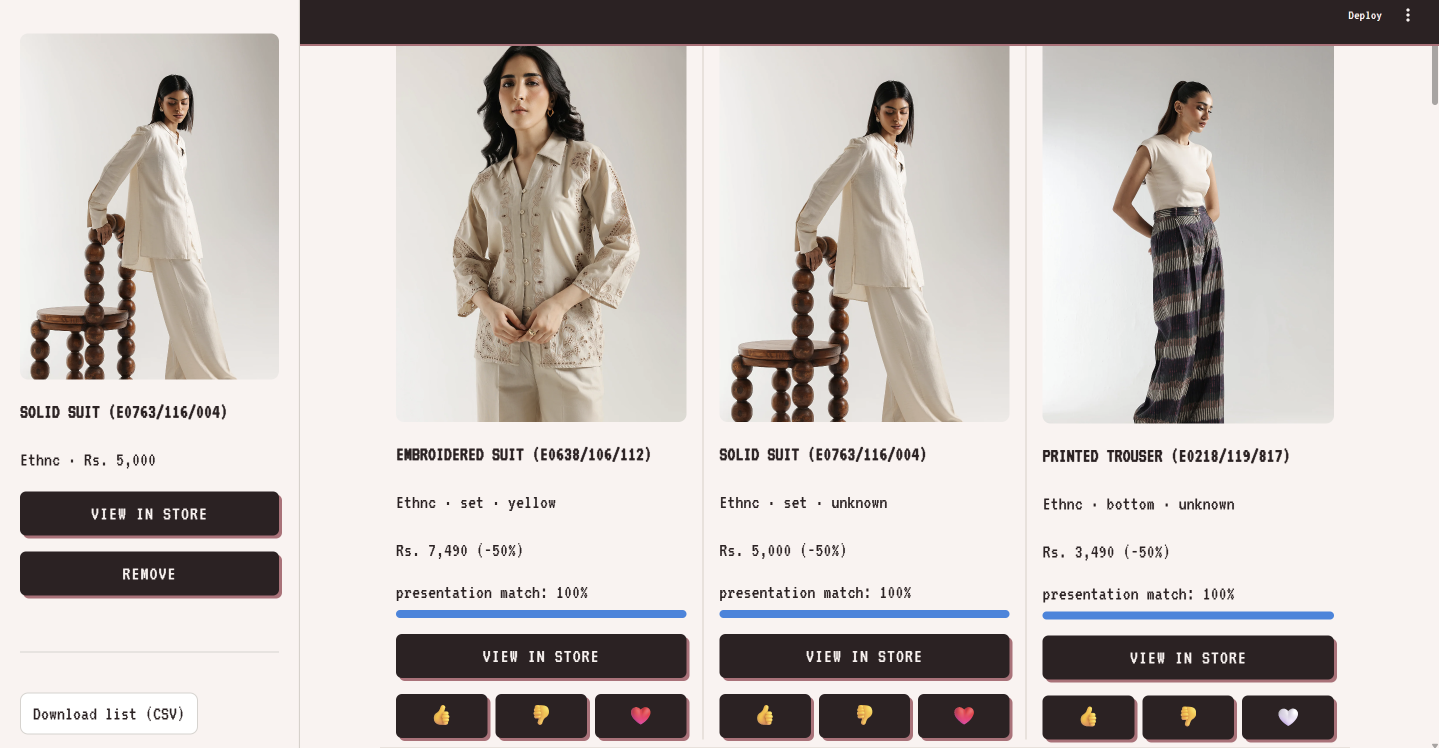
\includegraphics[width=\linewidth]{../figures/app_results.png}
  \caption{Results page for the occasion ``presentation'' with no colour filter. Each card has a store link and thumbs-up, thumbs-down and save buttons; the sidebar on the left shows a saved outfit with its remove button and the CSV download.}
\end{figure}}{\textbf{[Missing figure: app\_results.png]}\par}

\IfFileExists{../figures/app_filters.png}{%
\begin{figure}[htbp]\centering
  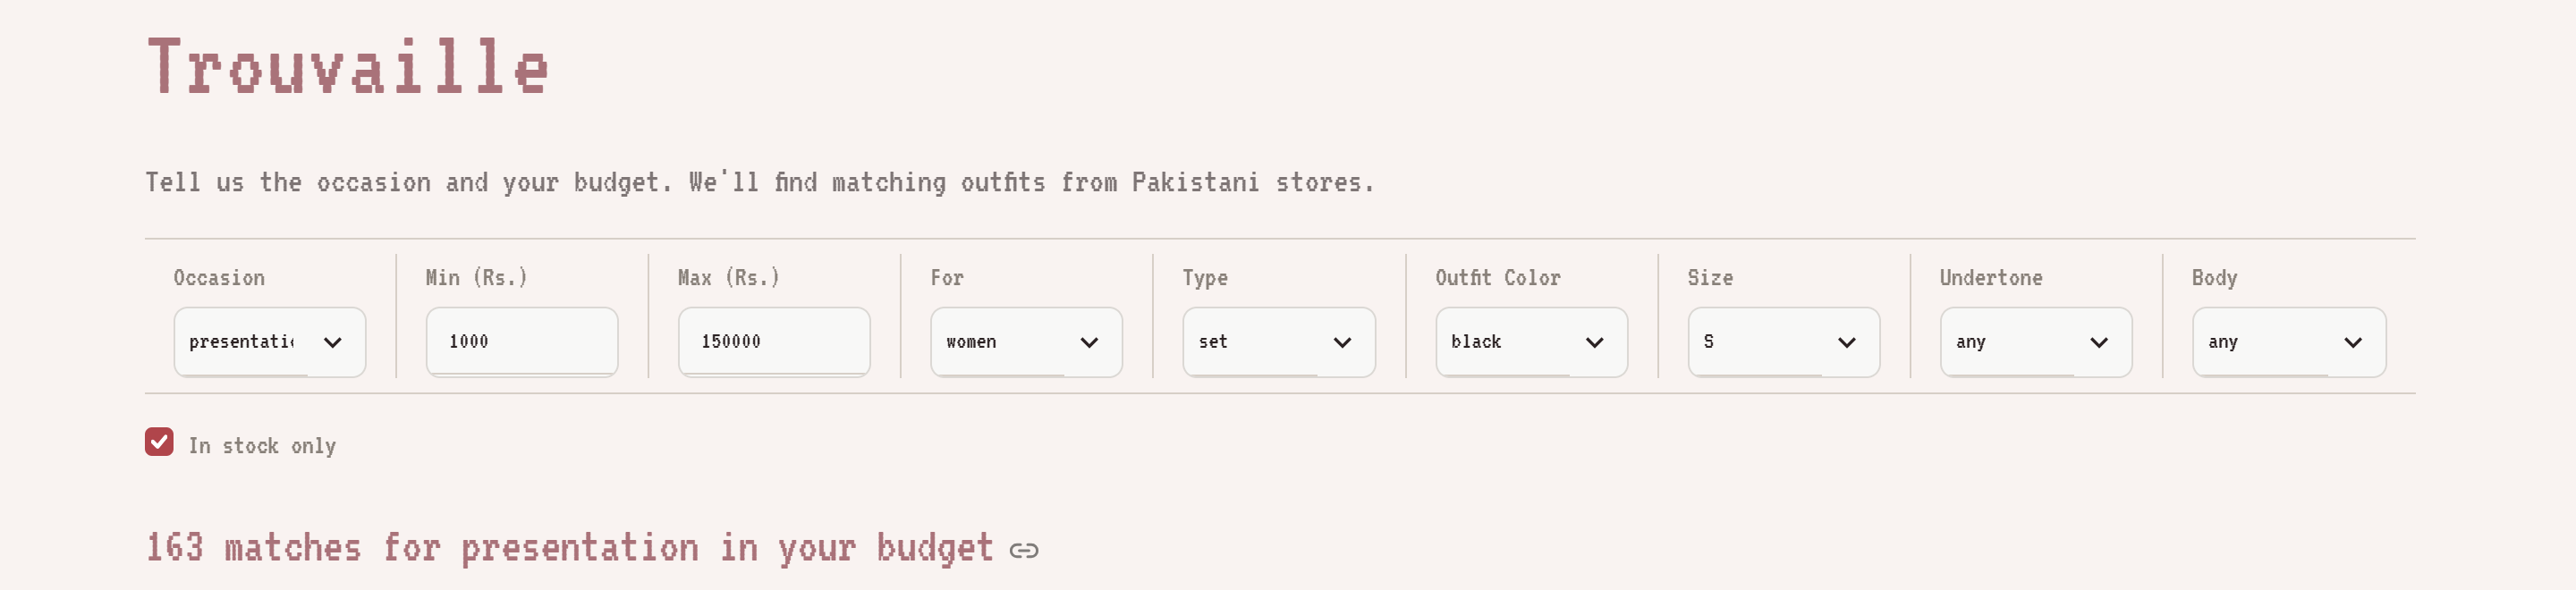
\includegraphics[width=\linewidth]{../figures/app_filters.png}
  \caption{The filter bar: occasion, minimum and maximum price, gender, type, outfit colour, size, undertone and body type, plus the in-stock checkbox. The line below it reports the number of matches (163 here).}
\end{figure}}{\textbf{[Missing figure: app\_filters.png]}\par}

\subsection{Sample Predictions}
Table~\ref{tab:samples} shows five searches run on the app's data (in stock only, probability of at least 0.5). The similarity is the cosine similarity between the typed text and the matched occasion.

\begin{table}[htbp]\centering\small
\begin{tabular}{p{2.6cm} p{2.5cm} p{1.5cm} p{5.6cm}}
\toprule
Search (budget) & Matched occasion (similarity) & Matches & Top result \\
\midrule
``graduation'' (Rs.~15{,}000) & presentation (0.52) & 4{,}332 & Ethnc, Printed Trouser, Rs.~3{,}490 \\
``wedding'' (Rs.~15{,}000) & wedding (0.59) & 4{,}167 & Outfitters, Relaxed Fit Washed Out Trousers, Rs.~4{,}890 \\
``office'', size M (Rs.~8{,}000) & office (0.60) & 2{,}352 & Ethnc, Printed Trouser, Rs.~3{,}490 \\
``party'' (Rs.~10{,}000) & concert (0.54) & 3{,}387 & J., Cream Lawn Digital Printed Unstitched 2Pc, Rs.~3{,}490 \\
``lehenga'' (Rs.~15{,}000) & wedding (0.14) & 4{,}167 & Rejected by the app (below the 0.25 cutoff) \\
\bottomrule
\end{tabular}
\caption{Sample searches. Counts are for the whole catalogue with no gender, type, color or other filters.}
\label{tab:samples}
\end{table}

The text matching behaves sensibly for phrases the model was not trained on: ``graduation'' maps to presentation and ``party'' to concert.
However, the ranking itself is weak. The top results often show a probability of about 100\%, so many products tie at the top and their order is not informative,
and some top results are hard to justify, such as washed-out trousers for a wedding.

\subsection{Result Discussion}
\paragraph{Why samples fail.} The occasion labels were produced by keyword rules, so the classifier largely learns to reproduce them; its high test score (macro F1 0.928) measures agreement with those rules, not with how a human would judge an outfit.
The model is also multi-label and gives high probabilities to several occasions for many products, which produces the ties and implausible top results seen above.
We did not investigate the cause further; noisy keyword labels are the most likely explanation, and hand-labelled data would be needed to confirm it.

\paragraph{Subgroup weaknesses.} The bias check on the test set showed lower macro F1 for some brands (Lama 0.695 on 68 items, Lulusar 0.765, Ethnc 0.867) than for others (Outfitters 0.971, Bonanza Satrangi 0.956),
and for some categories (tops 0.855, accessories 0.860, bottoms 0.878) than for sets (0.957). Unisex items (0.879) scored below men's (0.950) and women's (0.943) items.
A plausible reason is that these brands and categories describe products differently, so the keyword rules fit them less well, but we did not test this.

\paragraph{The ``lehenga'' query.} Searching for ``lehenga'' returned no results. The catalogue contains no product with ``lehenga'' in its title, and the query's similarity to the closest occasion (0.14) is below the app's cutoff, so the app asks the user to rephrase.
This is consistent with the data limitation that the luxury and bridal segment is almost absent from the scraped brands.

\subsection{Limitations and Future Work}
\begin{itemize}
  \item The app is run locally and is not hosted online.
  \item The size filter shows products that offer a size, not whether that size is in stock, because the scraped data holds only a product-level availability flag.
  \item Occasion labels, undertone matching and body-type filtering are heuristics. There is no learned skin-tone or body-type model, and no product ratings were collected. The thumbs-up/down feedback is stored in a local file, was only tried with a handful of test votes, and has not been evaluated; on a hosted deployment it would need persistent storage.
  \item The original project goal also included LLM query parsing, ratings-based re-ranking, an outfit builder and a Vibe Check Engine. These are not implemented; the app filters and ranks single products.
  \item Ranking is coarse: many products tie near 100\%, and results are not personalised. The feedback adjustment is capped at $\pm0.2$, so it only reorders products that are already close in score. The saved-outfits list is lost when the page is refreshed.
  \item The data is a single snapshot from eight effective brands, taken during a sale period, and kids' wear, luxury and bridal wear are largely missing.
  \item Future work: hosting the app online, hand-labelled evaluation data, per-variant stock scraping, a calibrated or fine-tuned model that separates occasions better, and learned undertone suitability.
\end{itemize}